\titre{}
\theme{}
\auteur{Nathan Scheinmann}
\niveau{}
\source{}
\type{serie}
\piments{1}
\pts{}
\annee{2526}

\contenu{
	\tcblower
\begin{center}
	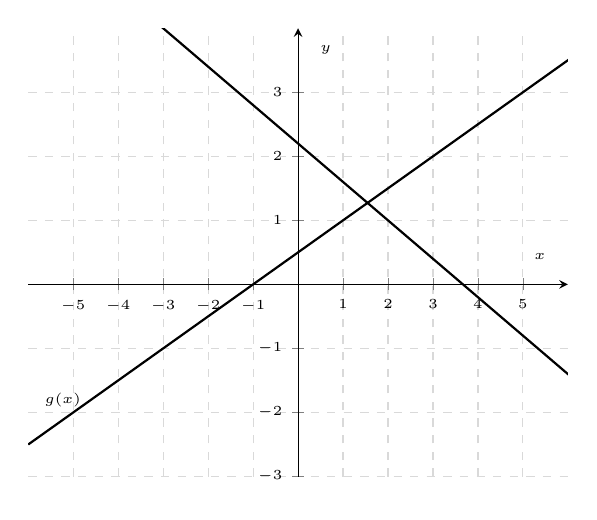
\begin{tikzpicture}[scale=1]
  \begin{axis}[
    axis lines=middle,
    xlabel={$x$}, ylabel={$y$},
    every axis x label/.style={at={(ticklabel* cs:0.92)}, anchor=west, yshift=10pt},
    every axis y label/.style={at={(ticklabel* cs:0.92)}, anchor=south, xshift=10pt},
    xmin=-6,   xmax=6,
    ymin=-3,   ymax=4,
    xtick={-5,-4,-3,-2,-1,0,1,2,3,4,5},
    ytick={-3,-2,-1,0,1,2,3},
    grid=both,
    grid style={dashed,gray!30},
    tick label style={font=\tiny},
    xlabel style={font=\tiny},
    ylabel style={font=\tiny}
  ]
    % branche pour x > 9
    \addplot[domain=-6:8, samples=200, thick]{-3/5*x+11/5}
      node[left,pos=0.1, font=\tiny] {$f(x)$};
    \addplot[domain=-6:8, samples=200, thick]{0.5*x+0.5}
      node[left,pos=0.1, font=\tiny] {$g(x)$};
  \end{axis}
\end{tikzpicture}
\end{center}
\begin{tasks}
\task Calculer les coordonnées du point d'intersection $I$ des deux droites
représentées ci-dessus.
\task Déterminer l'expression de la fonction $h$ qui passe par le point $I$ et
l'origine.
\task Déterminer l'expression de la fonction $i$ qui représente une droite
parallèle à $h$ passant par le point $P(2;-1)$.
  \end{tasks}

}
\correction{
	\tcblower

}
